\chapter{Results and Discussion}
\section*{3D Environment Reconstructions}
\begin{figure}[H]
    \centering
    \begin{subfigure}[b]{0.49\linewidth}
        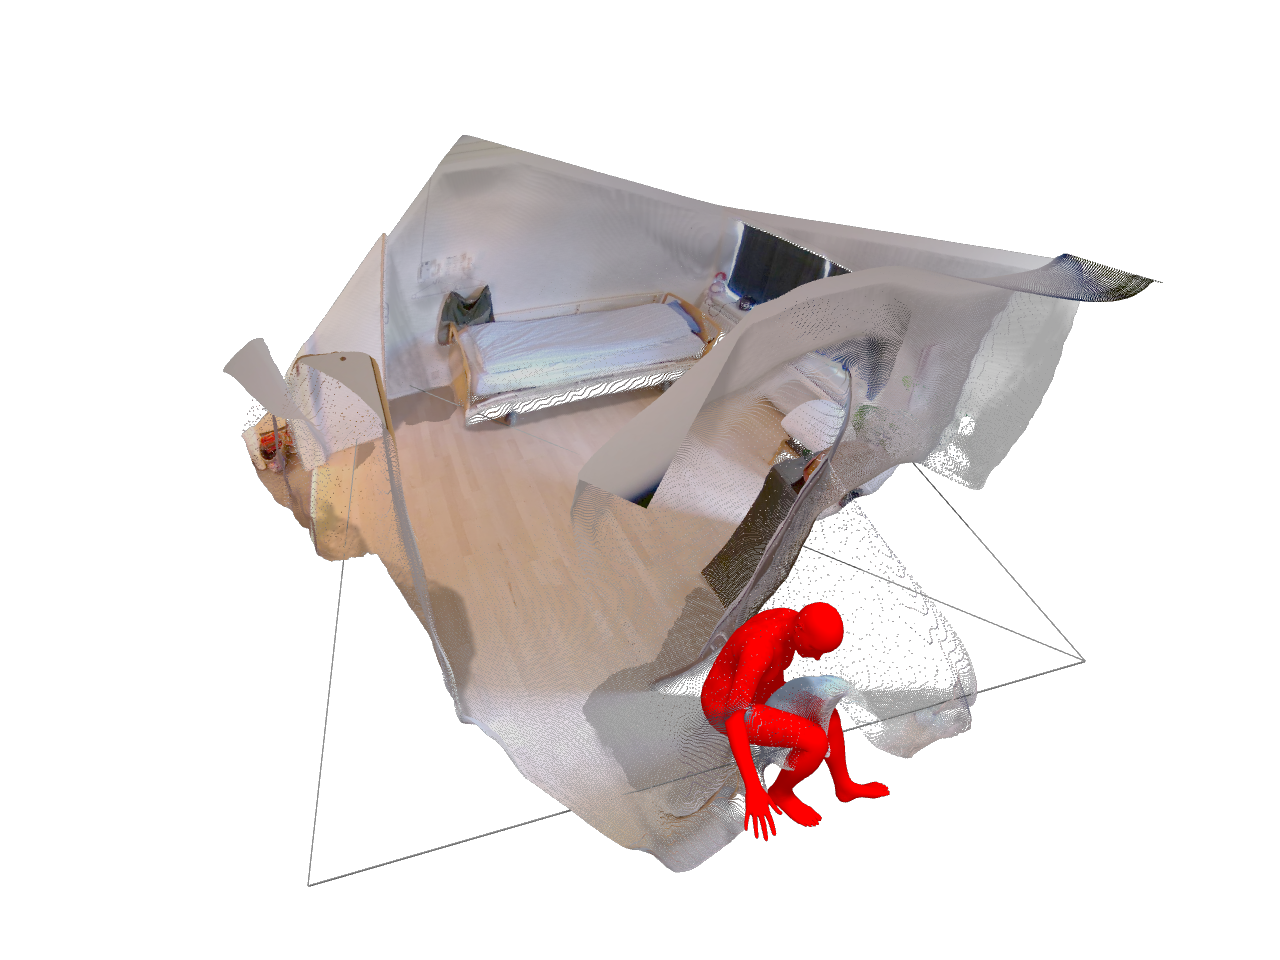
\includegraphics[width=\linewidth]{figures/results/room2.png}
    \end{subfigure}
    \hfill
    \begin{subfigure}[b]{0.49\linewidth}
        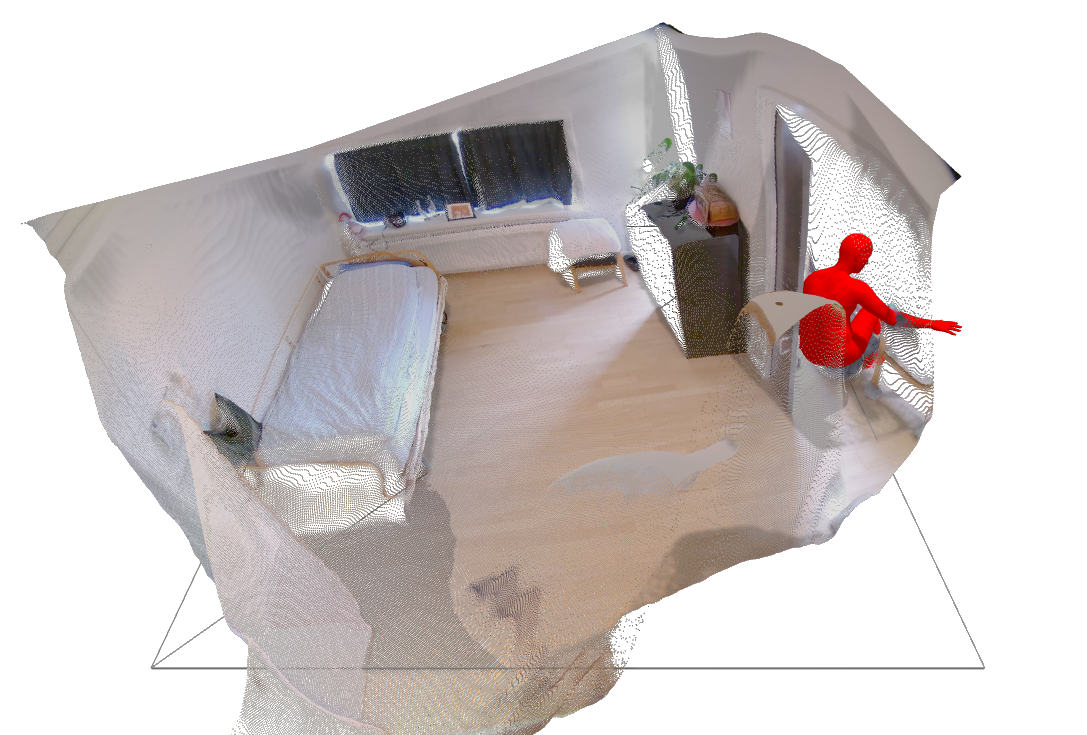
\includegraphics[width=\linewidth]{figures/results/room1.png}
    \end{subfigure}
    \caption{The person correctly positioned behind the door.}
    \label{fig:room1}
\end{figure}

\begin{figure}[H]
    \centering
    \begin{subfigure}[b]{0.49\linewidth}
        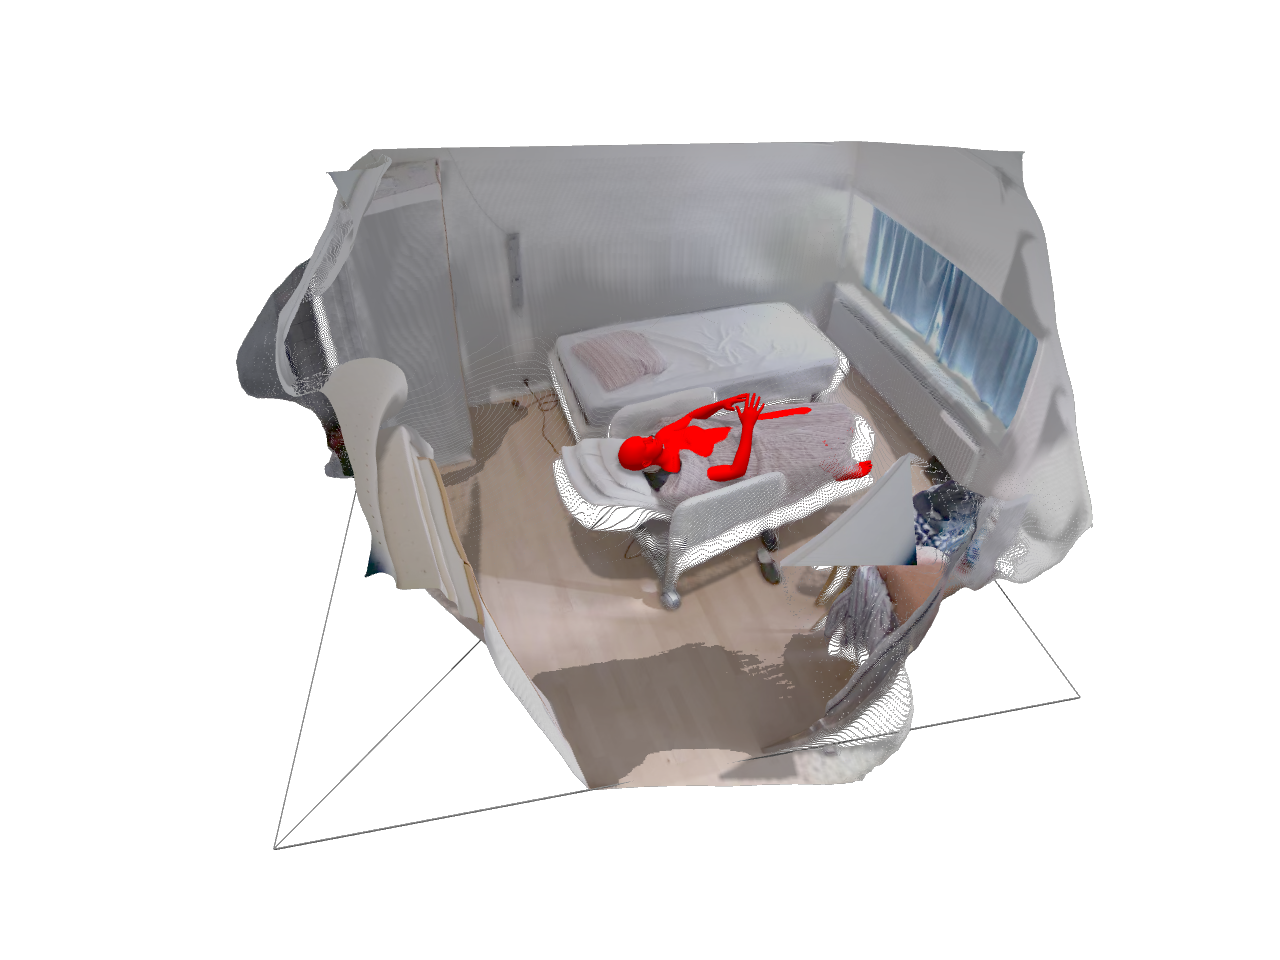
\includegraphics[width=\linewidth]{figures/results/room3.png}
    \end{subfigure}
    \hfill
    \begin{subfigure}[b]{0.49\linewidth}
        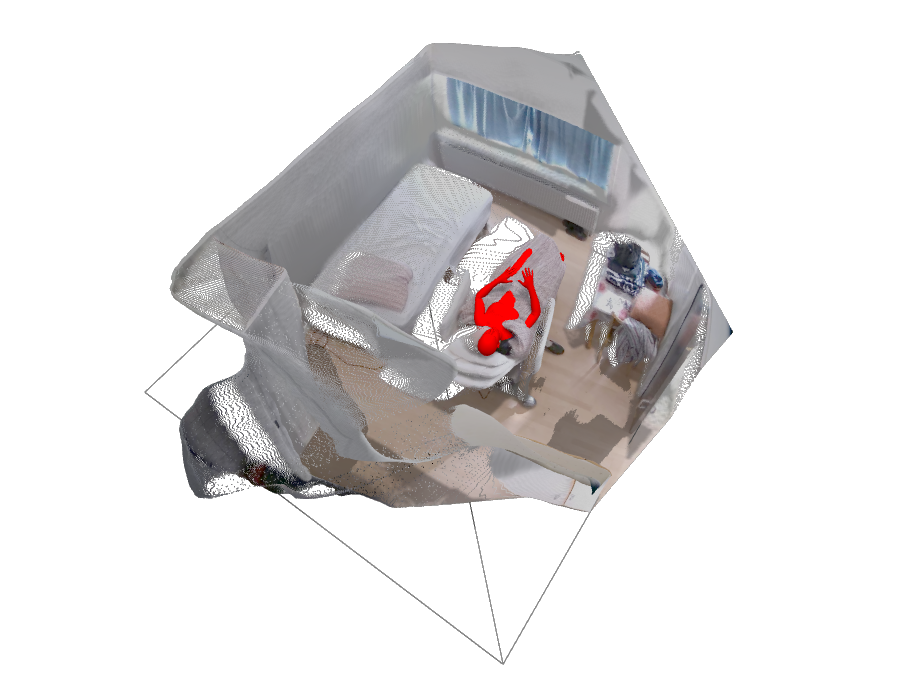
\includegraphics[width=\linewidth]{figures/results/room4.png}
    \end{subfigure}
    \caption{The person is accurately positioned in the bed.}
    \label{fig:room2}
\end{figure}
From visual inspection, we observe that we successfully reconstruct the coarse 3D geometry of the scene, align the floor plane to the XY-plane in the global coordinate system, and accurately populate the scene with our estimated poses. For example, in \cref{fig:room1}, the partially occluded person in the image is correctly placed behind the door. Similarly, in \cref{fig:room2}, the person is correctly positioned in the bed and even appears to be covered by the blanket. Additionally, we notice in the upper left corner of \cref{fig:room2} that the angles of the closet all seem to be around 90 degrees. These results suggest the feasibility and advancement of monocular depth estimation in restoring point clouds for indoor scenes. 


\section*{Motion Estimation}
\begin{figure}[H]
    \centering
    \includegraphics[width=0.9\linewidth]{figures/results/motion1.png}
    \caption{Example of bad annotations effect on estimated motion.}
    \label{fig:motion1}
\end{figure}

\begin{figure}[H]
    \centering
    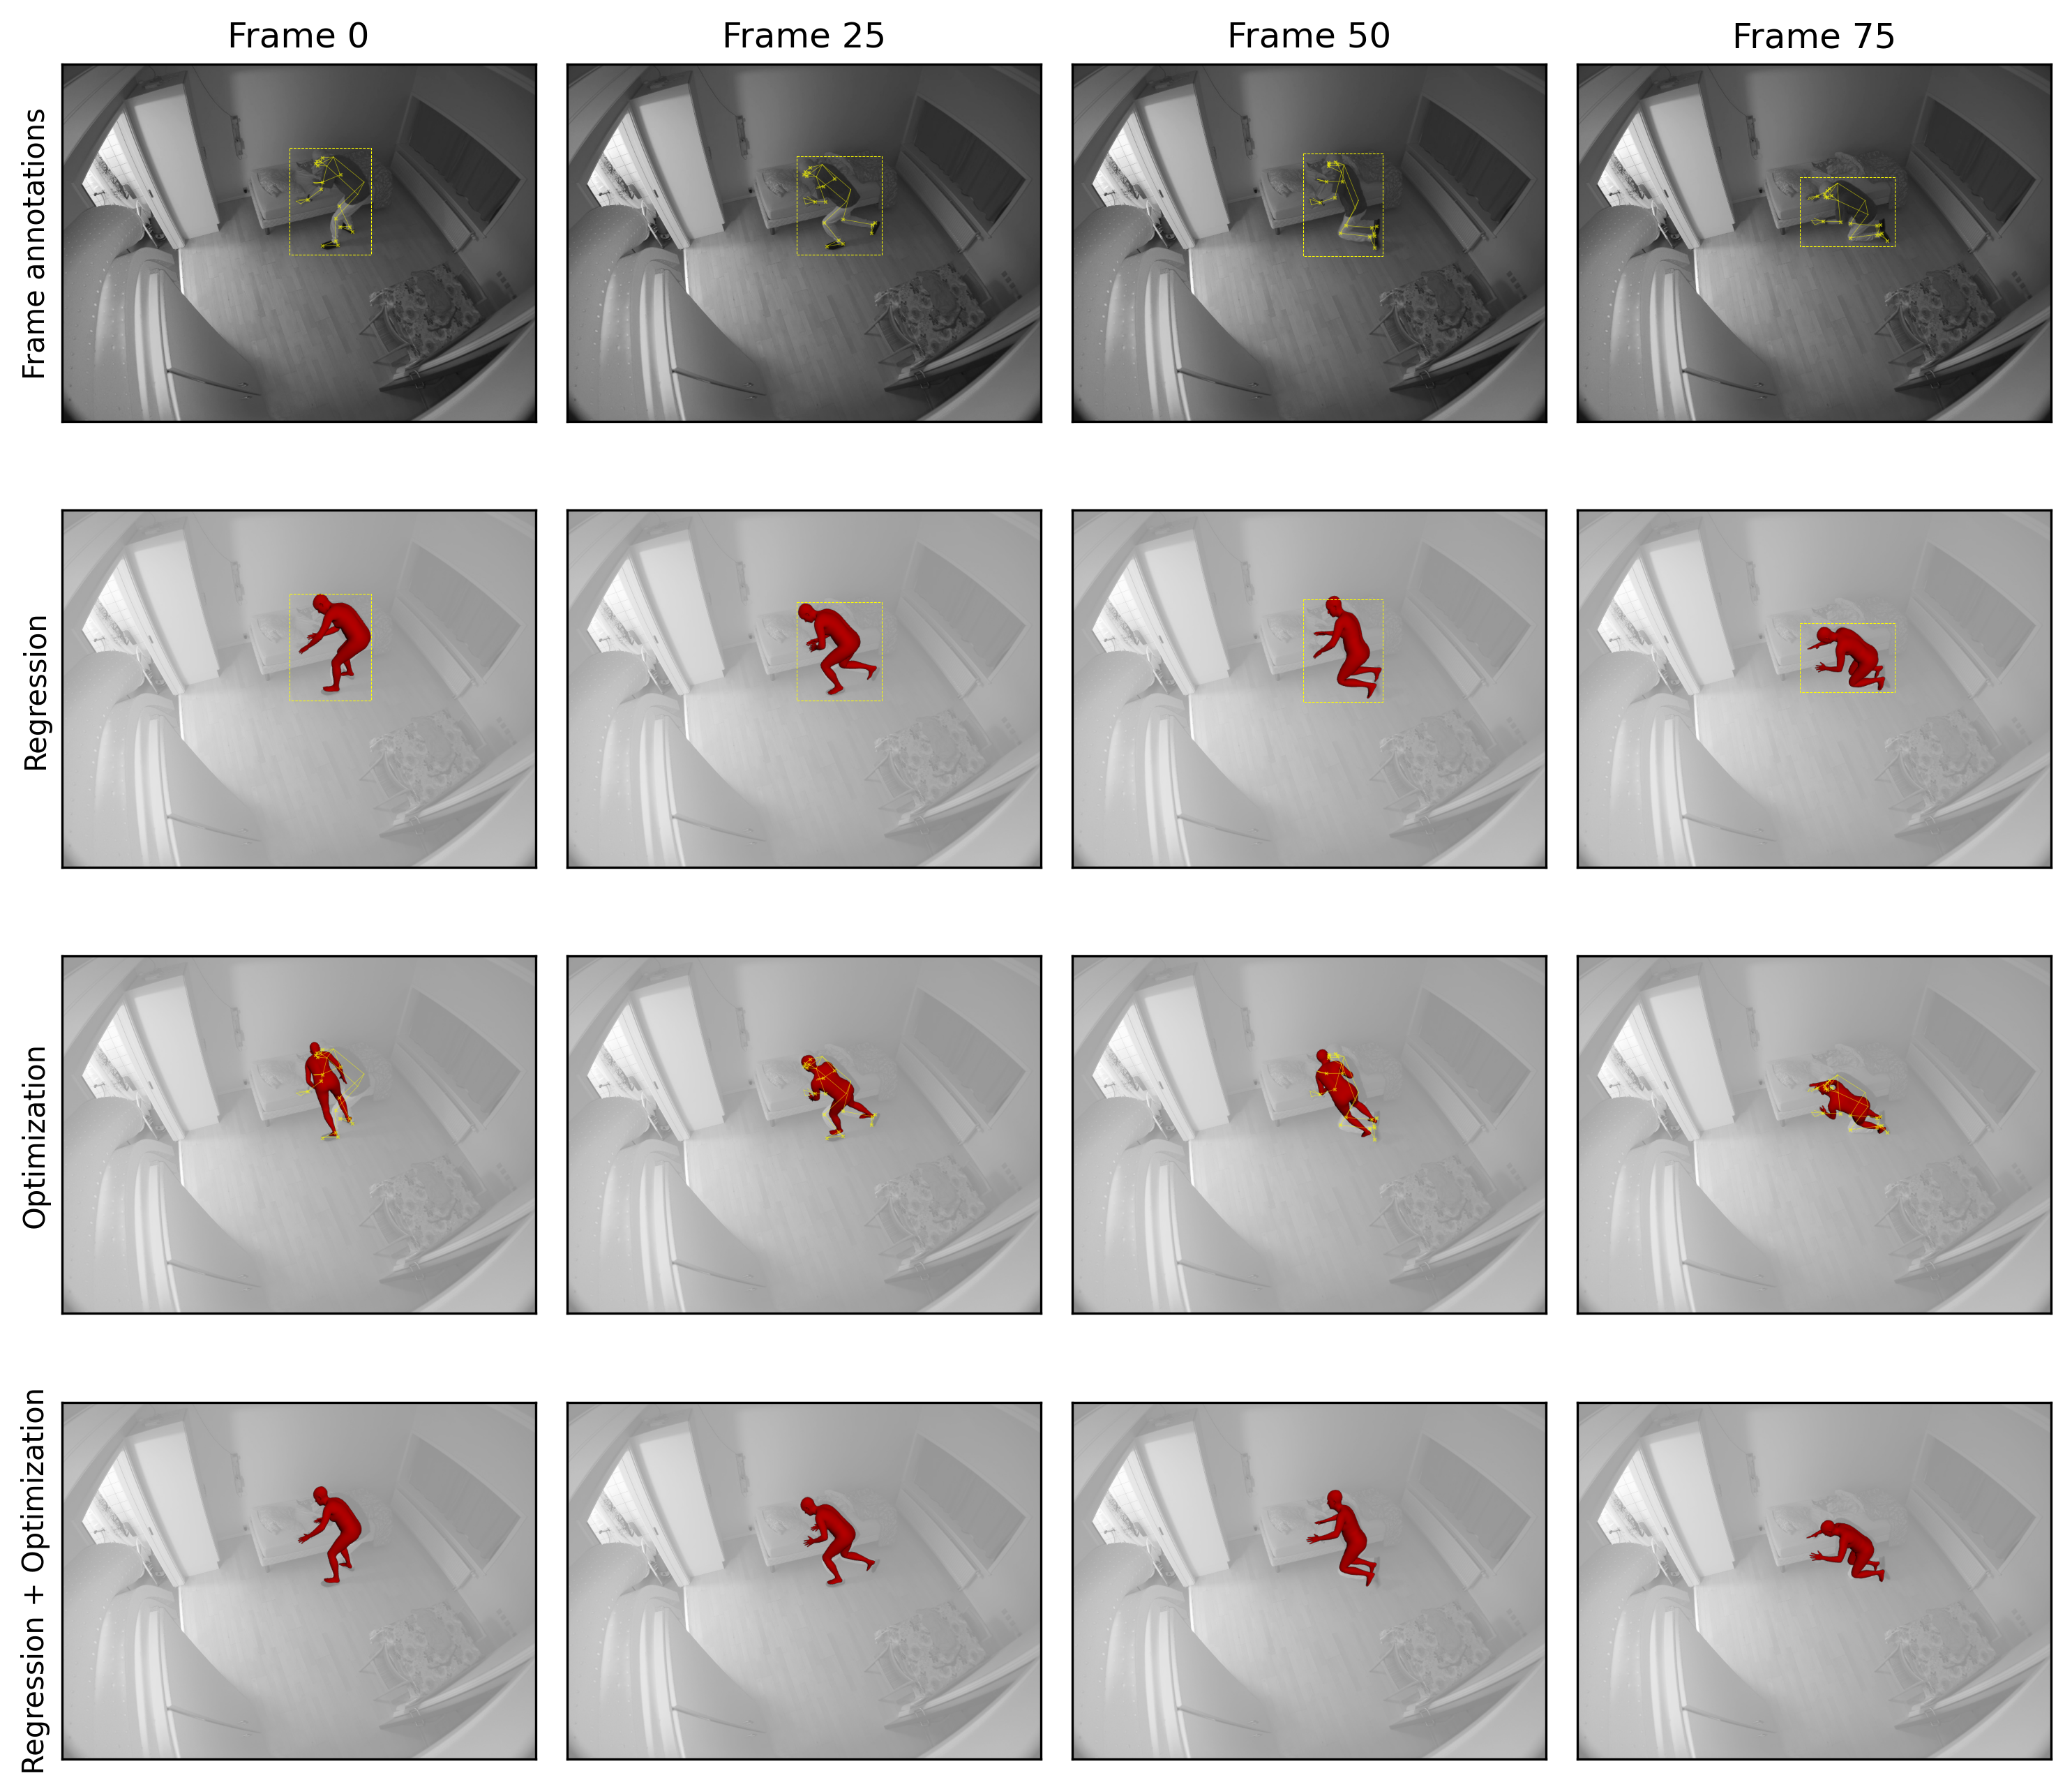
\includegraphics[width=0.9\linewidth]{figures/results/motion2.png}
    \caption{Local optimum of optimization-based method and hybrid method.}
    \label{fig:motion2}
\end{figure}

\begin{figure}[H]
    \centering
    \includegraphics[width=0.9\linewidth]{figures/results/motion3.png}
    \caption{Interpenetration between different people.}
    \label{fig:motion3}
\end{figure}

In the example shown in \cref{fig:motion1}, we notice that the keypoints do not correspond to the actual joints of the person. Specifically, the leg keypoints appear to be incorrectly marked as if the legs were covered by a blanket, despite being visible in the image, as indicated by the red ring. This might be an error in the keypoint annotations, either due to the autolabelling step in the pipeline failing to correctly detect the keypoints or a lack of human attention. As a result, the optimized pose (red) diverges from the actual pose of the person, while the green person's pose looks consistent with the person in the frame. Interestingly, the regressed pose also estimates the legs as being covered by the blanket, although it predicts the pose directly from the image. This again seems to be a result of a bad bounding box segmentation, not including the legs.

A common encountered problem with the optimization-based method is seen in \cref{fig:motion2}, where the optimized pose appears to be stuck in a local optimum during the optimization phase. In contrast, the regression-based method seems to correctly predict the pose but either overestimates the size of the person or places the person too close to the camera. Inspecting the outline of the person in the first frame indicates that the regression-based method might be sensitive to clothing or body shape. Initializing the pose from the regression estimates and then optimizing against the keypoints seems to give the best pose fit. 

As each pose is optimized in isolation, artifacts such as interpenetration might occur, as observed in the last row of \cref{fig:motion3}, after optimizing the initial regression-based estimate to align with the keypoints. Furthermore, the regression-based method fails to detect the occluded nurse behind the bed, as indicated by the semi-transparent mesh, indicating that the pose was removed due to closer matching the keypoints of the laying patient (see \cref{section:regression-pose-estimation}).

Overall, the examples show different trade-offs between regression- and optimization-based methods, with hybrid methods optimizing an initial regressed pose seemingly striking a good balance. However, more careful quantative evaluation is needed before making any final conclusions. 


% \begin{figure}[H]
%     \centering
%     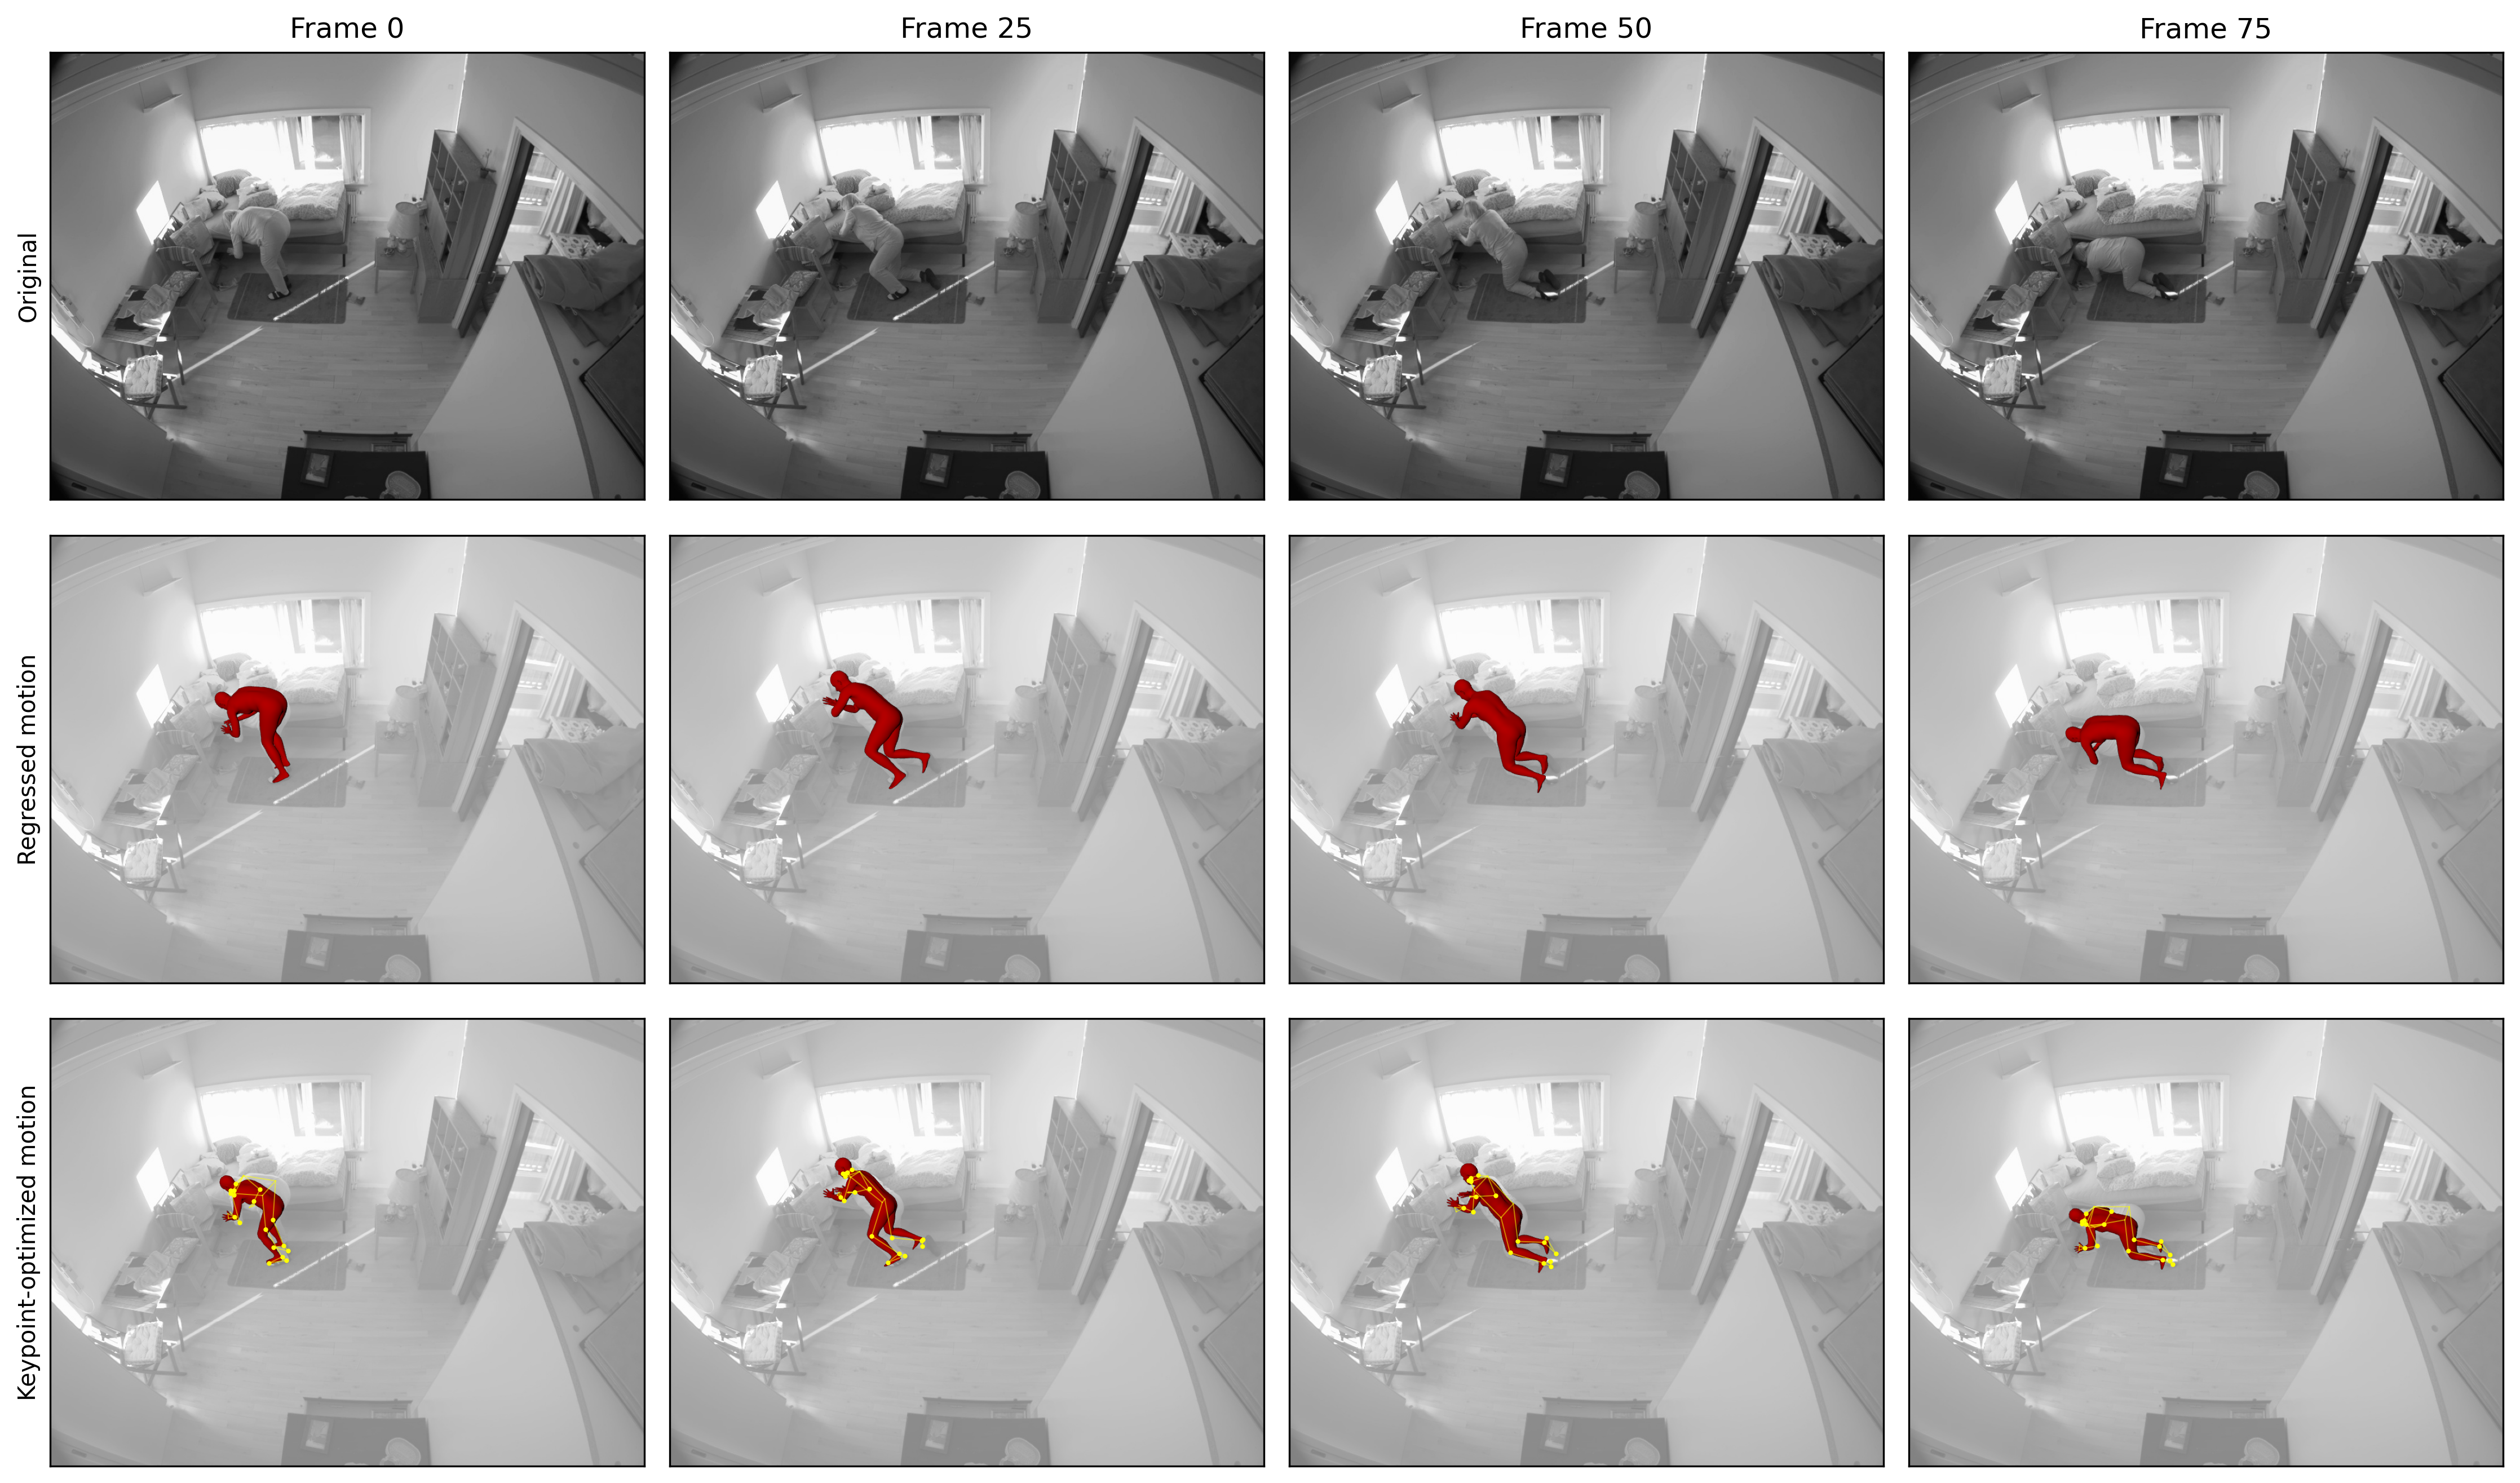
\includegraphics[width=\linewidth]{figures/results/motion4.png}
%     \caption{Example of bad ground truth kpts.}
% \end{figure}

% \begin{figure}[H]
%     \centering
%     \includegraphics[width=\linewidth]{figures/results/motion5.png}
%     \caption{Example of bad ground truth kpts.}
% \end{figure}

\section*{Single-Human Motion Generation}
\begin{figure}[H]
    \centering
    \begin{subfigure}{0.32\linewidth}
        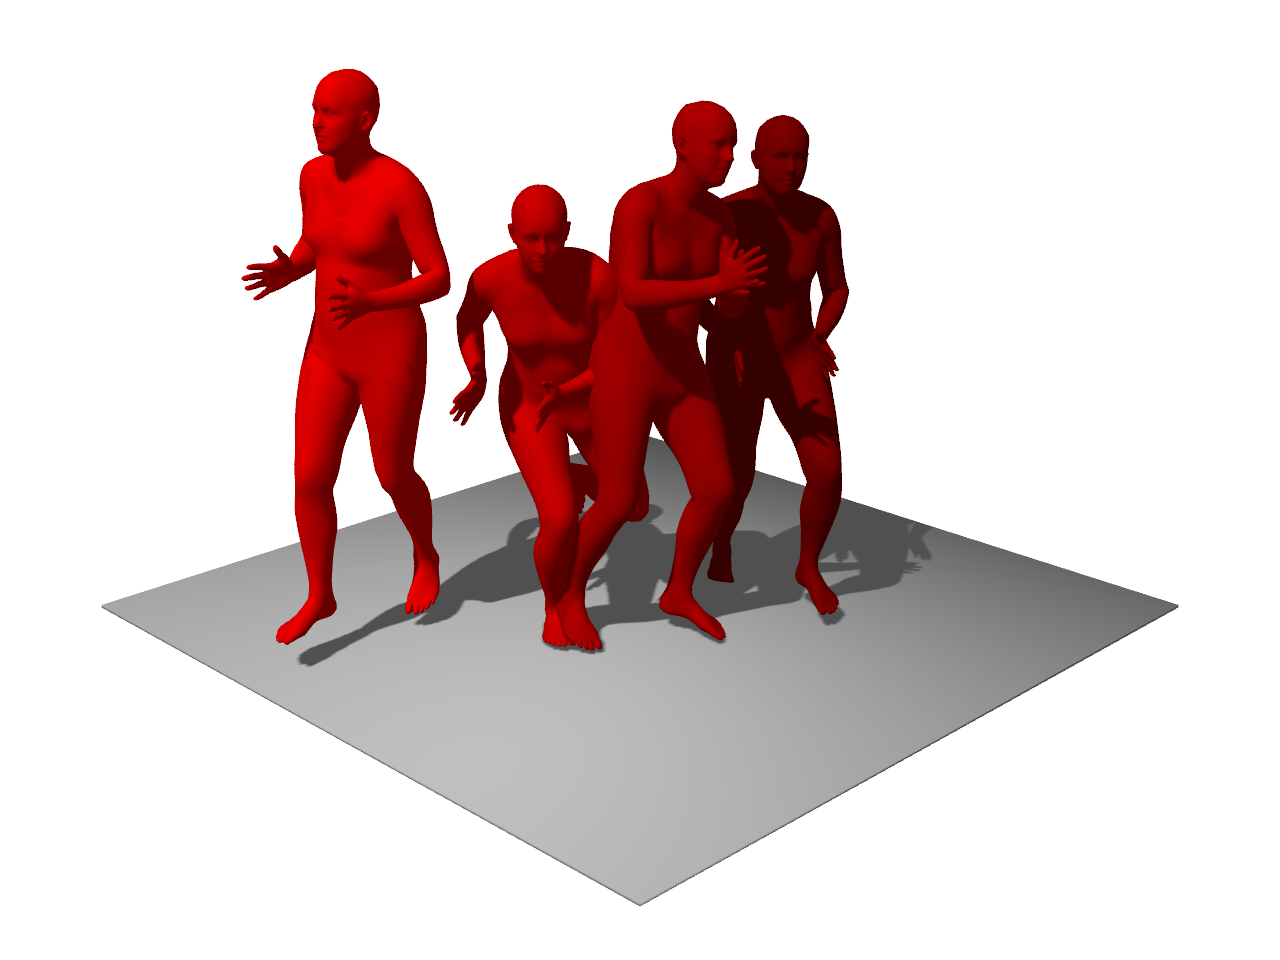
\includegraphics[width=\linewidth]{figures/results/single-kick1.png}
    \end{subfigure}
    \hfill
    \begin{subfigure}{0.32\linewidth}
        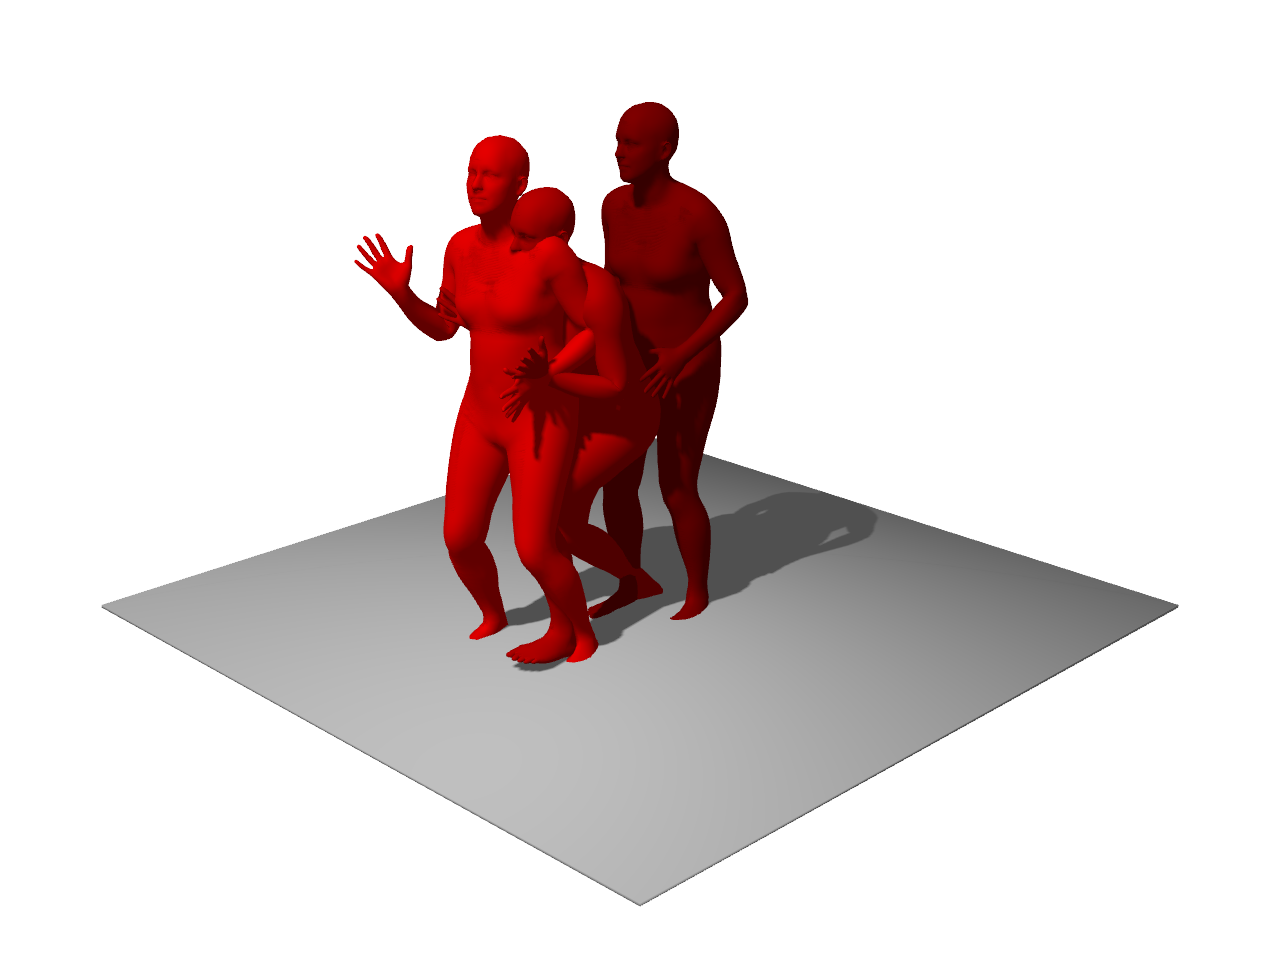
\includegraphics[width=\linewidth]{figures/results/single-kick2.png}
    \end{subfigure}
    \hfill
    \begin{subfigure}{0.32\linewidth}
        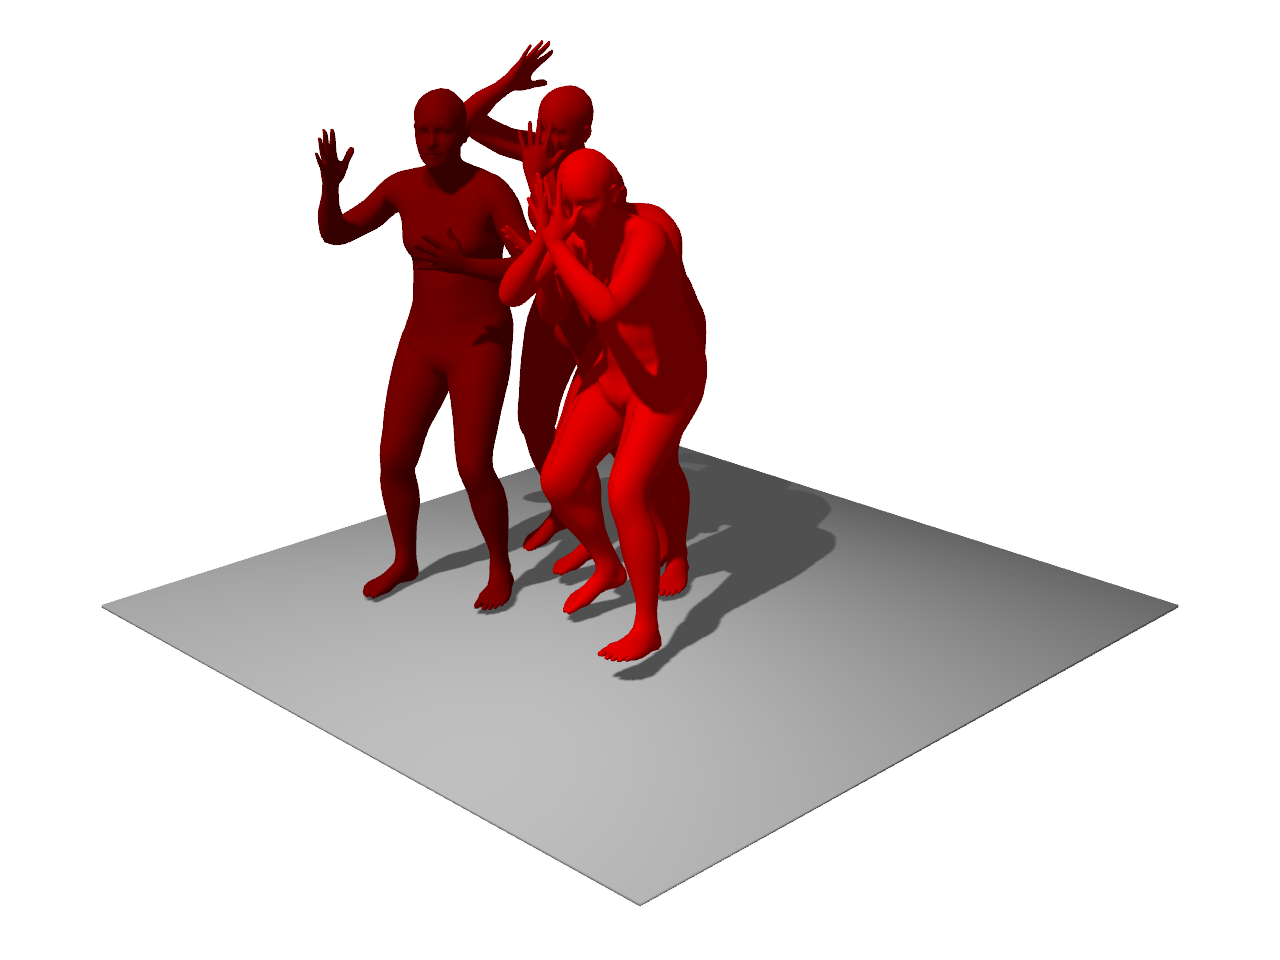
\includegraphics[width=\linewidth]{figures/results/single-kick3.png}
    \end{subfigure}
    \caption{\textit{"A person kicks with their left leg."}}
    \label{fig:single-kicks}
\end{figure}

\begin{figure}[H]
    \centering
    \begin{subfigure}{0.32\linewidth}
        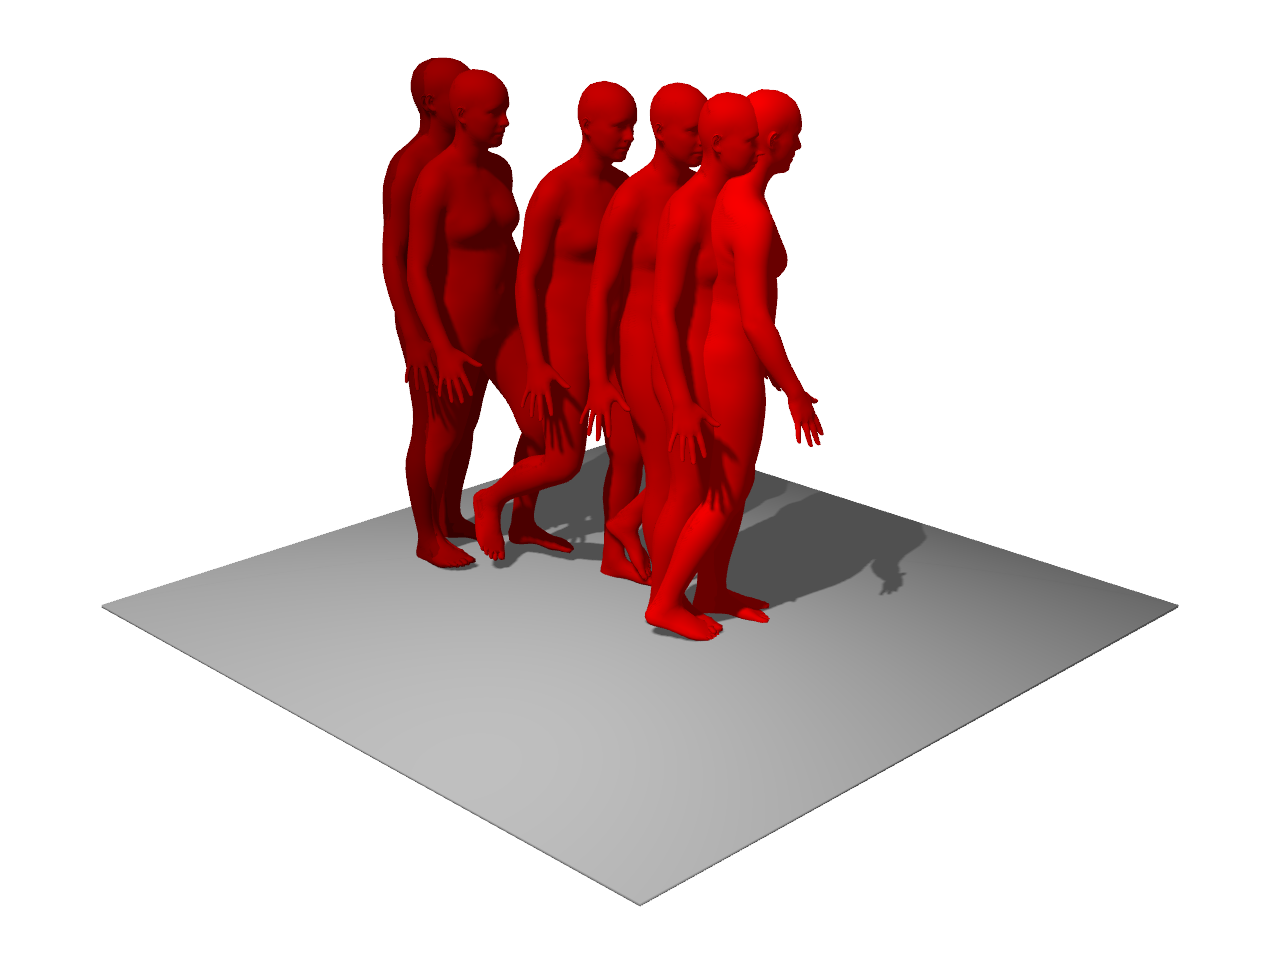
\includegraphics[width=\linewidth]{figures/results/single-runs1.png}
    \end{subfigure}
    \hfill
    \begin{subfigure}{0.32\linewidth}
        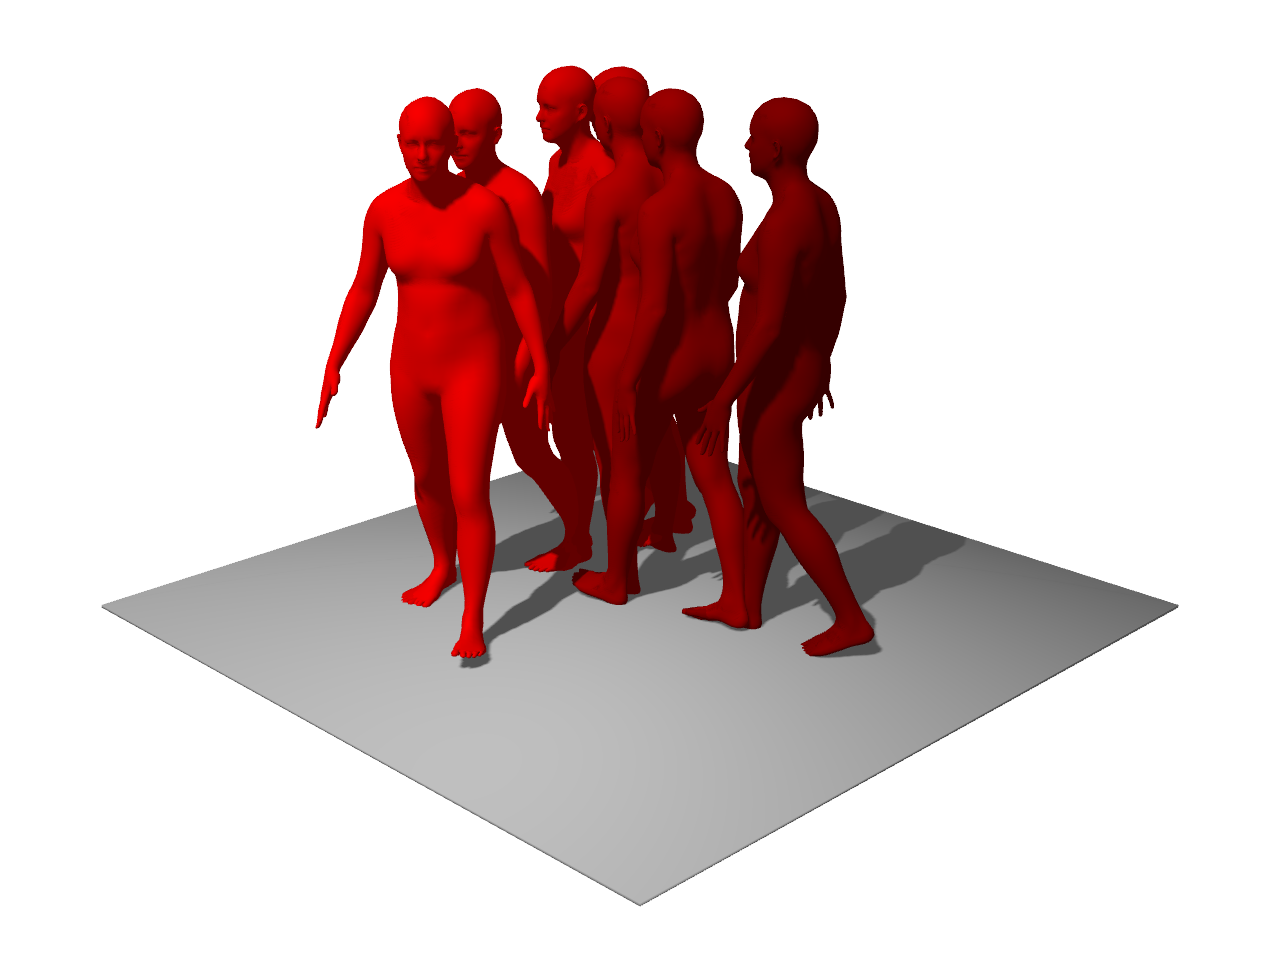
\includegraphics[width=\linewidth]{figures/results/single-runs2.png}
    \end{subfigure}
    \hfill
    \begin{subfigure}{0.32\linewidth}
        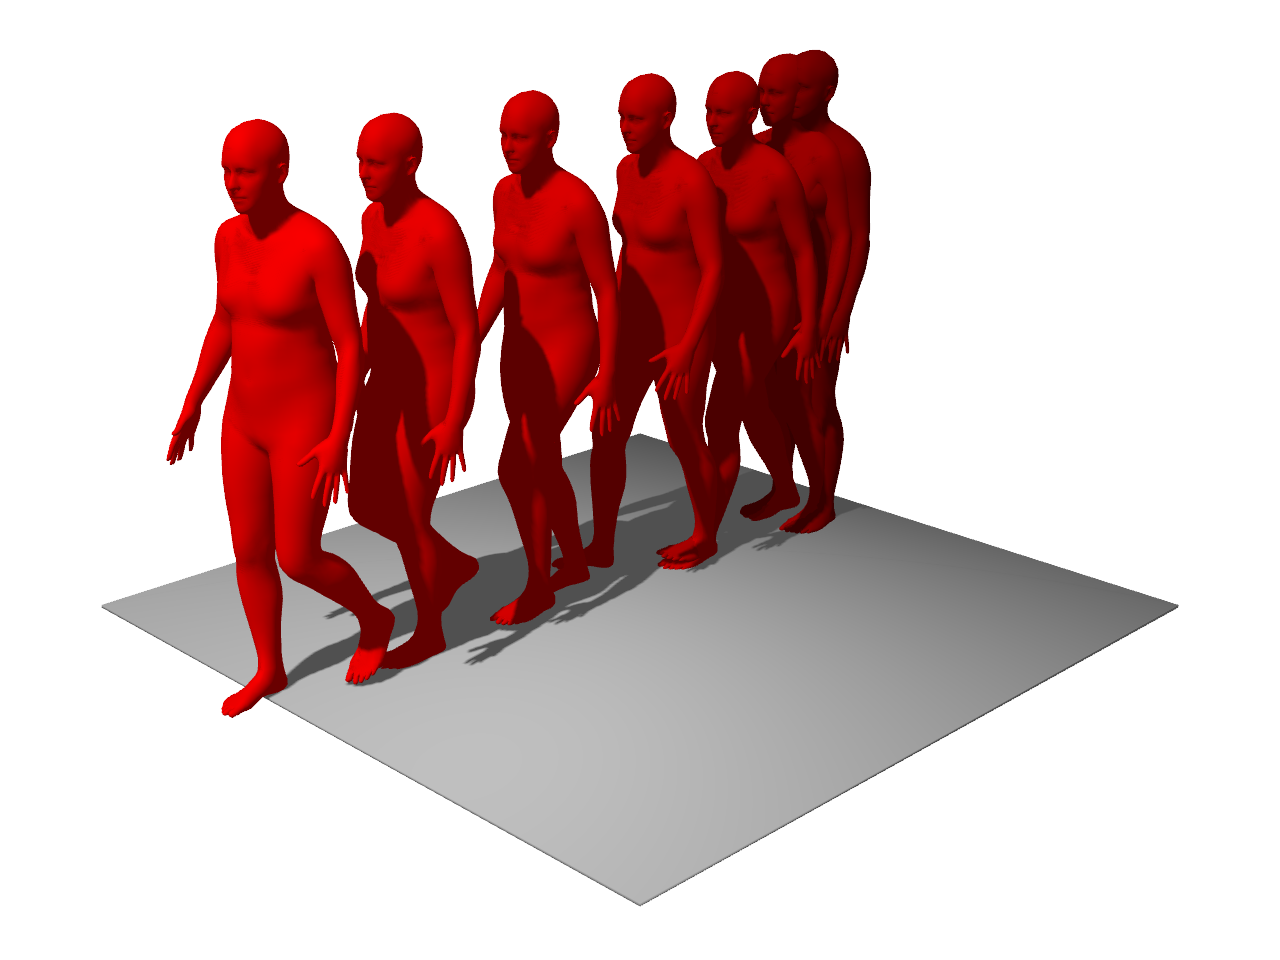
\includegraphics[width=\linewidth]{figures/results/single-runs3.png}
    \end{subfigure}
    \caption{\textit{"A man runs to the right then runs to the left then back to the middle."}}
    \label{fig:single-runs}
\end{figure}

\begin{figure}[H]
    \centering
    \begin{subfigure}{0.32\linewidth}
        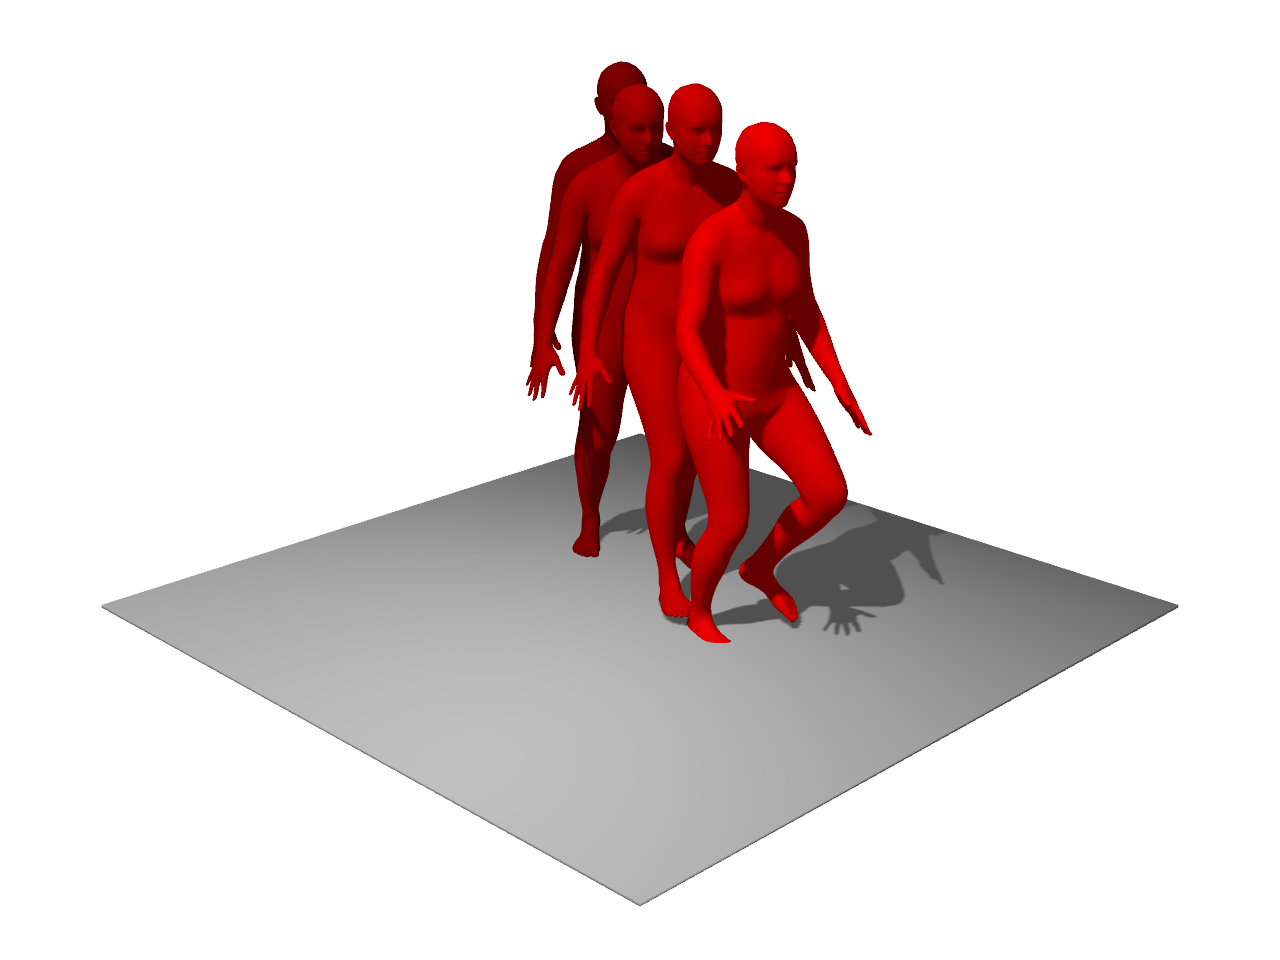
\includegraphics[width=\linewidth]{figures/results/single-falls1.png}
    \end{subfigure}
    \hfill
    \begin{subfigure}{0.32\linewidth}
        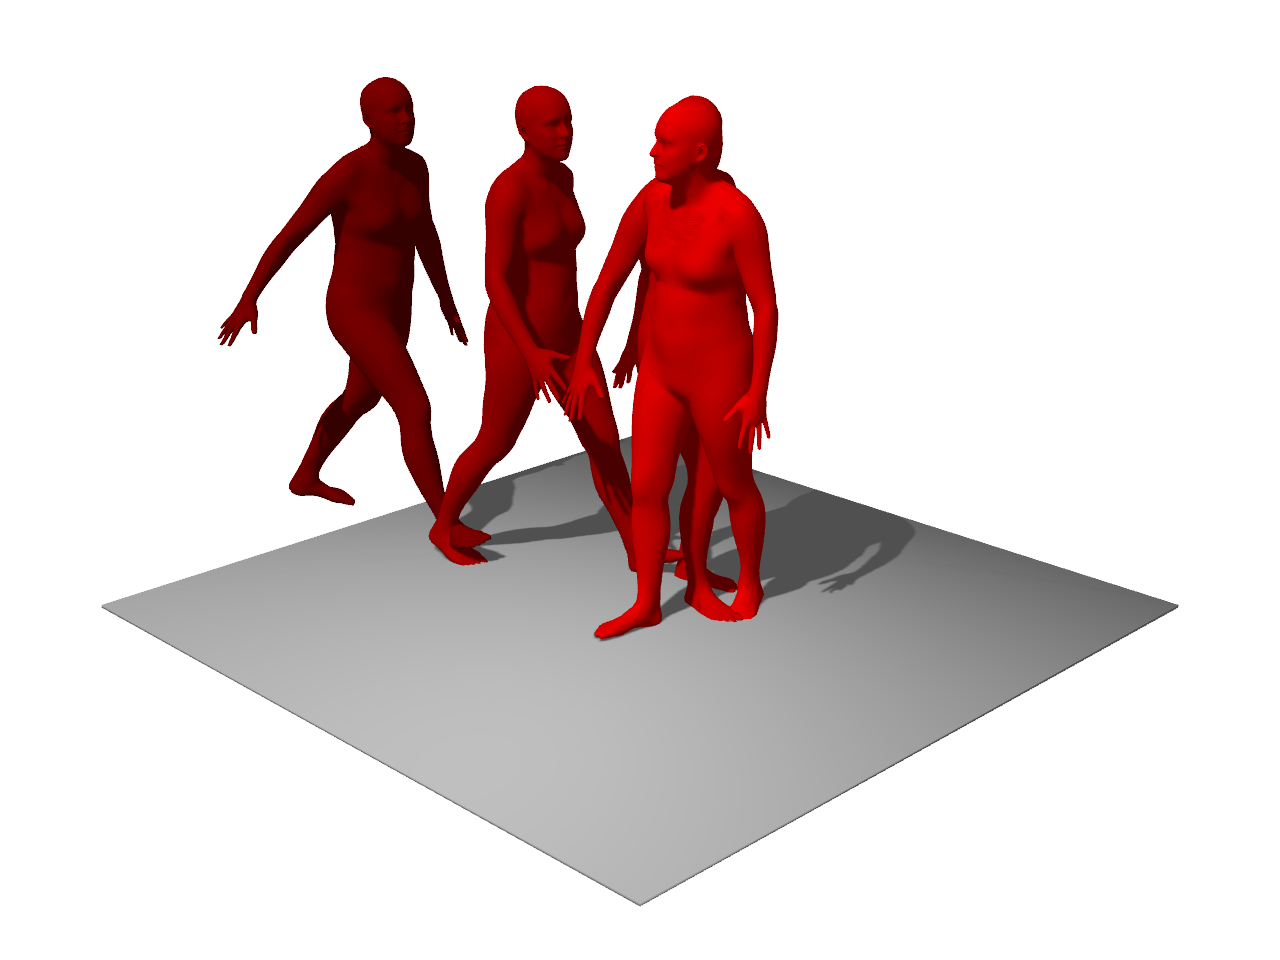
\includegraphics[width=\linewidth]{figures/results/single-falls2.png}
    \end{subfigure}
    \hfill
    \begin{subfigure}{0.32\linewidth}
        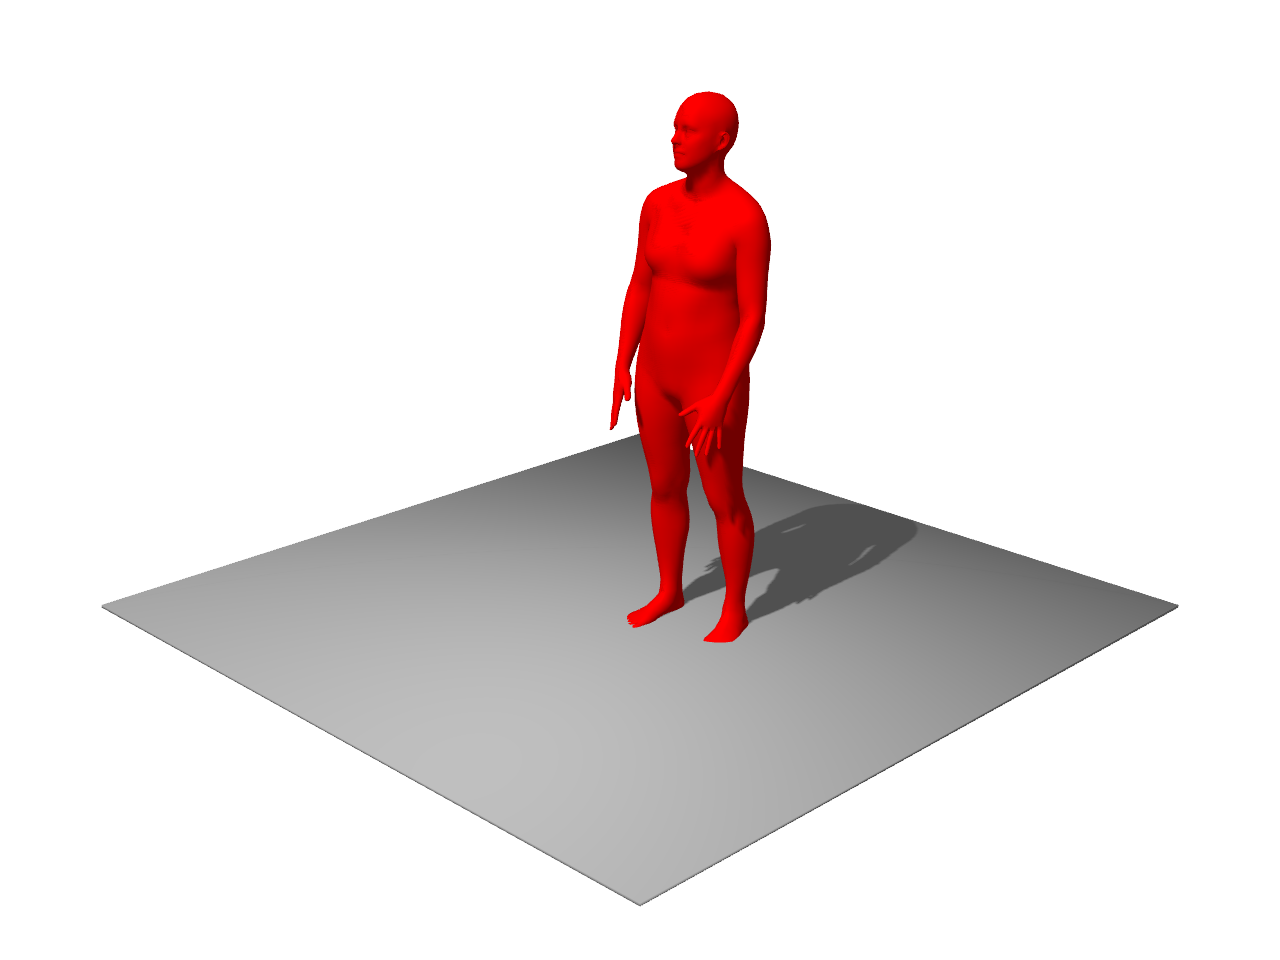
\includegraphics[width=\linewidth]{figures/results/single-falls3.png}
    \end{subfigure}
    \caption{\textit{"A person loses balance and falls to the ground."}}
    \label{fig:single-fall}
\end{figure}

We present three examples of single human motion generated from our proposed motion diffusion model, each conditioned on different prompts. For each prompt, we randomly sample three examples to illustrate the diversity of the generation. We sample motion sequence lenghts of 2s, 5s and 2s for each example, respectively. Following InterGen, sampling is performed using 50 DDIM steps with a classfier-free guidance weight of 3.5.

In the first example in \cref{fig:single-kicks}, we notice that none of the three motions seem to perform a kick as prompted; instead, they appear to defend against a kick if anything. This might suggest that the model hasn't fully learned the relationship between the prompt and the assignment of actions to individuals when generating single-human motion. One might want to model the assignment of actions more explicitly for more flexibility and control. 

In the second example in \cref{fig:single-runs}, all three sampled motions struggle to follow the prompted trajectory. Since the prompt is encoded into a single feature vector, it may be difficult for the model to comprehend promps featuring lists of tasks. It might be more effective to dynamically extract sub tasks from the prompt and base the motion generation on these. 

The last example (\cref{fig:single-fall}) of generated single-human motion also fails to perform the task of falling to the ground. This could be due to the model being biased towards standing positions, as these are most likely more prevalent in the training data. 

In general, the model seems able to generate realistic single human motion, but fails to perform the action given in the prompt or misassign the given task by instead performing the counterpart reaction, as if another individual was performing the prompted task. We tried increasing the classifier-free guidance scale to 10 and 12 to see if this would steer the model more towards the desired motion, but found it to only improve adherence slightly while resulting in more chaotic and unrealistic motion. 

Due to limited time, that model was only trained for 500 epochs and did not seem to have fully converged. One could expect further improvements by training longer, for the conditional part of the network to better learn the correlation between the description embedding and the resulting motion.


\section*{Dual-Human Motion Generation}

\begin{figure}[H]
    \centering
    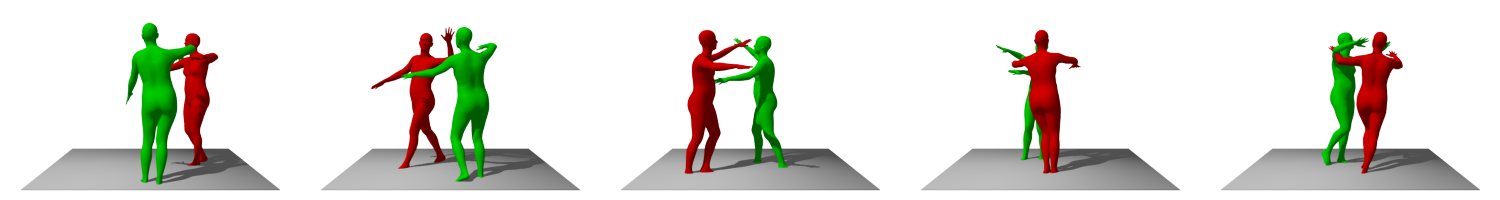
\includegraphics[width=\linewidth]{figures/results/multi-passion.png}
    \caption{\textit{"With fiery passion two dancers entwine in Latin dance sublime."}}
\end{figure}


\begin{figure}[H]
    \centering
    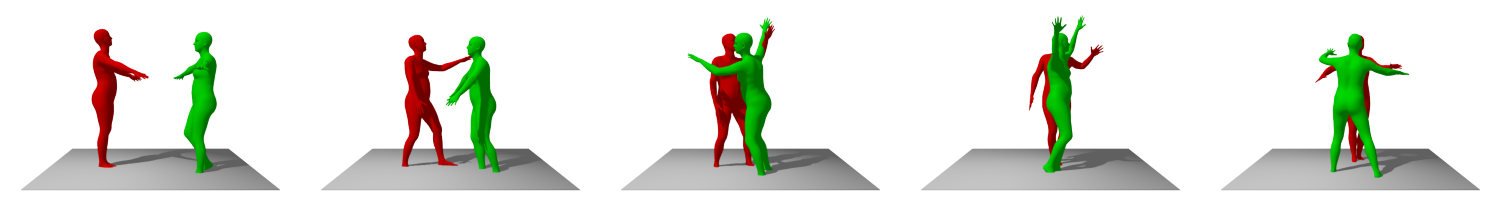
\includegraphics[width=\linewidth]{figures/results/multi-selfie.png}
    \caption{\textit{"With merry smiles the two snap their selfie."}}
\end{figure}


\begin{figure}[H]
    \centering
    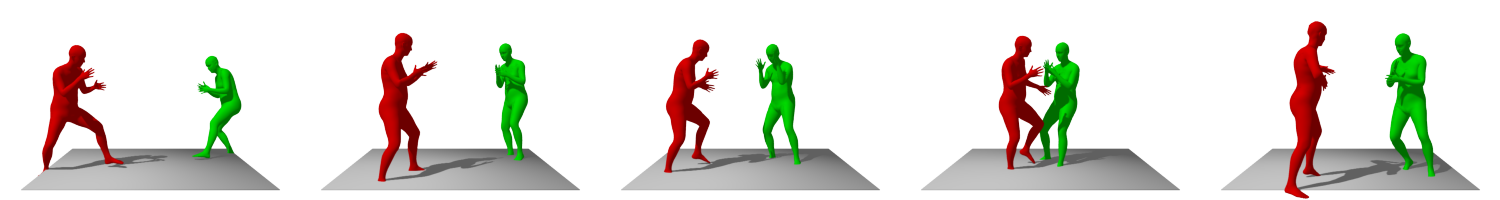
\includegraphics[width=\linewidth]{figures/results/multi-pick-up.png}
    \caption{\textit{"Two people picking up something from the ground."}}
\end{figure}

We first test our model's ability to generate two-person motion and present three randomly selected examples of generated interactions. Again, we observe that, except for the first example, the generated motions, although realistic, do not follow the given prompts. We attempt to regenerate the motion with increased guidance scales of 7.0 and 10.0, but this does not improve adherence. Interestingly, for all guidance scales, the prompt “Two people picking up something from the ground” results in generated motion that resembles a fighting scene. 


\subsection*{Multi-Human Motion Generation}

\begin{figure}[H]
    \centering
    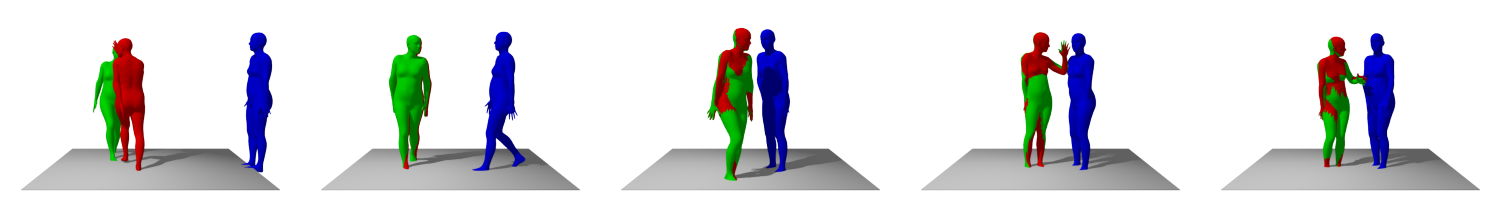
\includegraphics[width=\linewidth]{figures/results/multi.png}
    \caption{\textit{"Three people are dancing around in a circle."}}
    \label{fig:multi1}
\end{figure}

\begin{figure}[H]
    \centering
    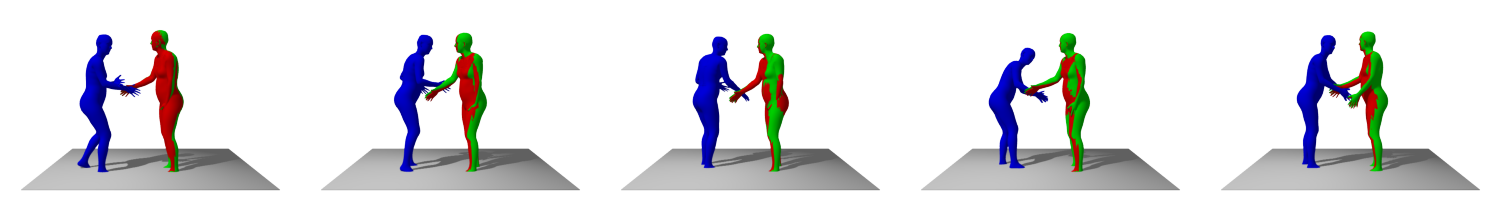
\includegraphics[width=\linewidth]{figures/results/multi2.png}
    \caption{\textit{"Two people shaking hands while the third person looks the other way."}}
    \label{fig:multi2}
\end{figure}

\begin{figure}[H]
    \centering
    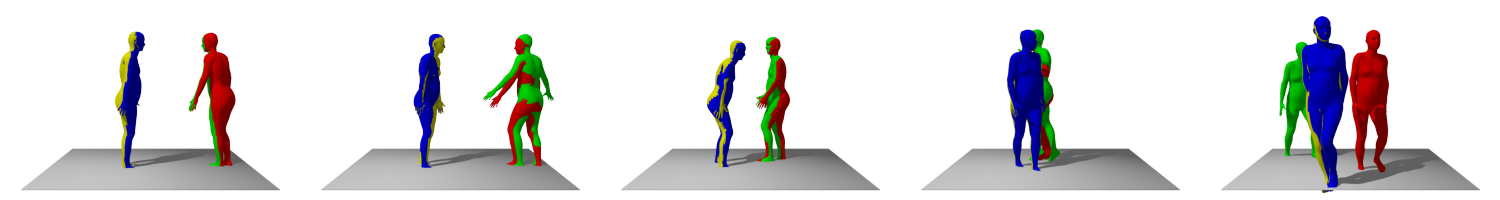
\includegraphics[width=\linewidth]{figures/results/multi3.png}
    \caption{\textit{"Four people walking in a straight line one after the other."}}
    \label{fig:multi3}
\end{figure}

When generating motions for more than two people, we observe that the model sometimes merges two individuals into one, sharing the same pose and location. This merging and unmerging occur in both directions, as shown in \cref{fig:motion1} and \cref{fig:motion3}, respectively. Adherence to prompts is generally lacking, except in \cref{fig:motion2}, where two people are correctly shaking hands as instructed. However, the third person is merged and therefore not looking away as expected.

It appears that the model currently differentiates identities based on joint positions rather than identity embeddings. This issue could potentially be resolved by training the model on multi-human interactions involving more than two people in crowded scenes, where an identity encoding would be more effective.

